\begin{abstract}
El lenguaje Gobstones posee una secuencia didáctica bien definida que ha demostrado ser eficaz tanto en cursos iniciales universitarios como en escuelas secundarias. En el marco de una comunidad creciente de usuarios, proponemos el desarrollo de un \textit{Entorno Integrado de Aprendizaje de Programación} a partir de una implementación de Gobstones sobre un \textit{Editor Proyectivo}, haciendo uso de sus cualidades intrínsecas para facilitarle al alumno la comunicación de soluciones en términos de conceptos en lugar de trabajar sobre texto plano, reduciendo así elementos superfluos que pudieran entorpecer la secuencia didáctica.
\end{abstract}



\section{Introducción}

En la República Argentina la enseñanza de la programación en el segundo ciclo primario y primer ciclo secundario se plantea utilizando lenguajes eminentemente visuales \cite{CuadernoDocenteProgramAR}. Esto permite a los alumnos concentrarse en aquello que desean expresar (es decir, el programa que pretenden crear) al eliminar ciertas dificultades inherentes en lenguajes sobre soporte de texto. Por ejemplo, el lenguaje Scratch\cite{scratch} únicamente permite construcciones \textit{sintácticamente válidas} ya que cada comando del lenguaje es conformado por bloques visuales encastrables, de tal manera que dos bloques solo encastran cuando constituyen una combinación válida.

Luego, cuando el alumno pasa a un ciclo superior secundario o a la universidad, se le presentan lenguajes basados en texto, en los cuales los errores de sintaxis y de tipado son posibles. En particular en la Universidad Nacional de Quilmes, en la materia de Introducción a la Programación, se utiliza el lenguaje Gobstones\cite{Gobstones}, creado específicamente para la enseñanza de programación.

Si bien Gobstones cuenta con un modelo acotado y una secuencia didáctica clara, que lo convierten en una gran herramienta para la enseñanza universitaria y de ciclos superiores del secundario; al ser basado en texto presenta un nivel de complejidad que puede no resultar adecuado para el segundo ciclo de la educación primaria o el primer ciclo de la educación secundaria.

En este contexto surge la propuesta de crear una implementación de Gobstones que permita únicamente sintaxis válida, de manera similar a los lenguajes visuales ya usados en la enseñanza de la programación, reduciendo así elementos superfluos que pudieran entorpecer la secuencia didáctica planteada para el segundo ciclo de la educación primaria y el primer ciclo de la educación secundaria.
Además, se presenta a esta implementación de Gobstones en un entorno que acompañe su secuencia didáctica, tanto desde la construcción de ejercicios y planteo de problemas, como la inclusión paulatina de conceptos nuevos durante el proceso de aprendizaje. Se pretende lograr una continuidad entre la enseñanza de la programación utilizando componentes visuales y texto, volviendo más gradual la transición entre uno y otro.


Para lograr esta experiencia cercana al texto pero con la ausencia de errores sintácticos, resulta idóneo el uso de un Editor Proyectivo, término acuñado por Martin Fowler en el año 2005\cite{Fowler} al intentar plantear un ambiente de desarrollo donde el programador pueda expresar sus ideas en términos de conceptos en lugar de texto. Lo que vemos como texto pasaría entonces a constituir una representación editable del concepto al que hace referencia (y al cual Fowler llama \textit{representación abstracta}). Los conceptos del lenguaje son el dominio de los editores proyectivos, y decimos que un programa es una \textit{representación abstracta} construida utilizando dichos conceptos. Para modificar esta representación el programador interactúa con una interfaz de usuario, llamada \textit{representación editable}, sobre la cual la \textit{representación abstracta} se \textit{proyecta} en forma de texto\cite{voelter2014projectional}. 

De esta manera, el editor solamente permite ingresar construcciones sintácticamente válidas en un formato estandarizado (espacios, identación y demás elementos estéticos son dados por el editor, no por el usuario).

En la sección \textit{II} se presenta la tecnología a usar y en la sección \textit{III} se describe el desarrollo del modelo conceptual del lenguaje Gobstones en términos de esa tecnología. En la sección \textit{IV} se muestra cómo este modelo conceptual se proyecta sobre el editor. Una vez creado el editor, se procede a implementar el intérprete del lenguaje y la renderización de los tableros inicial y final. Teniendo el lenguaje básico funcionando, se trabaja en la sección \textit{V} sobre el sistema de inferencia de tipos, orientado a asistir al estudiante mediante mensajes de error legibles. En la sección \textit{VI} se analizan problemas típicos de los editores proyectivos y se busca mejorar la experiencia de usuario aplicando diferentes técnicas que facilitan una edición más familiar, es decir, más cercana a una expriencia de edición de texto. Luego en la sección \textit{VII} se extiende el proyecto agregando un \textit{lenguaje de definición de ejercicios}, que constituye un lenguaje específico de dominio cuya finalidad es permitirle al docente plantear ejercicios, desde título y descripción hasta restriciones de features de lenguaje y análisis de código. Por último en la sección \textit{VIII} se cierra el informe con una conclusión e ideas sobre el camino que el proyecto pudiera seguir a futuro.

\section{Tecnología proyectiva a usar}

De los entornos proyectivos existentes hoy en día, se decide utilizar el workbench Meta Programming System (MPS)\cite{MPS} de la empresa Jetbrains, en su versión 3.3.
Se trata de un entorno orientado al desarrollo de lenguajes maduro y estable, sobre el cual se realizaron exitosamente diferentes proyectos, entre los cuales se cuentan:
\begin{itemize}
\item MetaR\cite{MetaR}: un IDE que utiliza el lenguaje R para facilitar el análisis de datos biológicos.
\item mbeddr\cite{mbeddr}: un IDE orientado a la programación sobre hardware, que extiende el lenguaje C y soporta verificación formal, máquinas de estado y variabilidad en líneas de productos, entre otros.
\item YouTrack\cite{YouTrack}: un gestor de proyectos.
\end{itemize}

MPS brinda un DSL para la definición de conceptos puros del lenguaje a implementar, y sobre estos la posibilidad de describir cómo este modelo se renderizará, comportamiento específico para cada concepto, sistema de tipos, etc. Al ser todas estas incumbencias transversales a los conceptos, se organizan en forma de aspectos.
Los conceptos se comportan de manera similar a una clase en programación orientada a objetos, en tanto y en cuanto admiten extensión por herencia e implementación de interfaces. A su vez, estas construcciones determinan las instancias de nodos que compondrán un programa, comparables a los nodos de un árbol de sintaxis abstracta.

A partir de los lenguajes definidos en esta herramienta es posible generar un IDE autónomo o pluguins para IDEs pre-existentes.

\section{Modelo conceptual del lenguaje Gobstones}

Se comienza modelando el lenguaje Gobstones en términos de conceptos. Como puede observarse en el ejemplo de \fig{ifElse_concept}, para cada concepto pueden definirse sus posibles nodos hijo, propiedades y referencias a otros nodos. Se organizan en una jerarquía, pudiendo extender de otros conceptos e implementar interfaces. En este caso, puede verse que el concepto \textit{IfElseStatement} extiende del concepto abstracto \textit{Statement}, y sus posibles hijos son una expresión, que será la condición de la alternativa, un bloque de sentencias para el caso en que la condición sea verdadera, y otro bloque de sentencias para el caso contrario.

\begin{figure}[hb]
\centering
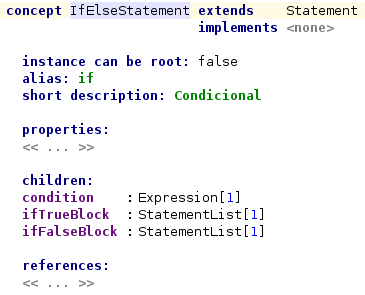
\includegraphics[width=0.4\textwidth]{assets/ifElse_concept}
\caption{Definición del concepto para la alternativa condicional}
\label{fig:ifElse_concept}
\end{figure}

Los conceptos más importantes serán \textit{Statement}, que denota un comando, y \textit{Expression} que denota una expresión que puede ser evaluada. De manera simplificada, tenemos que el primer nivel de la jerarquía de sentencias queda dado por:

\Tree [.Statement 
    Alternative 
    Loop
    Procedure
    Assignment
].Statement 
\bigskip

Y el primer nivel de la jerarquía de expresiones se compone de:

\Tree [.Expression 
    BinaryOperation 
    Value 
    Function
].Expression 
\bigskip

Además, se tiene una jerarquía separada para la definición de rutinas:

\Tree [.RoutineDeclaration 
    ProcedureDeclaration 
    FunctionDeclaration
].RoutineDeclaration 
\bigskip

Decimos entonces que un programa gobstones básico se encuentra dado por una colección de sentencias y una colección de definición de rutinas.

Donde el siguiente programa:

\begin{lstlisting}[frame=single] 

program {
  Poner(Rojo)
}

function verdadero(){
  return(True)
}
    
\end{lstlisting}

Corresponde a un modelo conceptual con la estructura:

\Tree [.Program 
    [.StatementsList
      [.NativeProcedure
        Red        
      ].NativeProcedure
    ].StatementsList
    [.FunctionDeclaration
      [.StatementsList
        Empty
      ].StatementsList
      True
    ].FunctionDeclaration
].Program 
\bigskip

\section{Implementación del Editor}

\section{Implementación del Intérprete}

\subsection{Edición del tablero inicial}

\subsection{Renderización del tablero final}

\section{Inferencia de tipos}

\section{Mejorando la experiencia de Usuario}

\subsection{Edición de operaciones binarias}
\subsection{Borrado de nodos}

\section{Lenguaje de Definición de Ejercicios}

\section{Conclusión}

\section{Anexo}
\subsection{Configuración de los proyectos}


\section{Introducción}

En esta sección se detallan brevemente las características del lenguaje Gobstones, se determina qué se entiende por \textit{Entorno Integrado de Aprendizaje de Programación} y se da una introducción al funcionamiento de los editores proyectivos.


\subsection{El lenguaje Gobstones}

Gobstones es un lenguaje de programación que fue diseñado para la enseñanza teniendo como elementos fundacionales de su filosofía: el desarrollo de la abstracción, el aprendizaje de la división de tareas y la obtención de pautas de estilo que favorezcan la posterior interpretación de los programas generados, todo manteniendo un alto grado de simplicidad conceptual y eliminando elementos superfluos que claramente complican el aprendizaje inicial. 
Actualmente es soportado por diversas herramientas, entre las cuales se destaca el editor \cite{PyGobstones}

\subsection{Entorno Integrado de Aprendizaje}

Los entornos integrados de aprendizaje\cite{IntegratedLearningEnvironment} cubren un gran número de herramientas. En el presente trabajo al hablar de \textit{Entorno Integrado de Aprendizaje de Programación}, de ahora en más \ile (\textit{Integrated Learning Environment}), nos referiremos a una aplicación diseñada para la enseñaza de la programación, orientada a cumplir cierta estrategia didáctica y facilitar la creación de planes de estudio por parte del docente. 

Es importante diferenciar al \ile de un \textit{IDE} (\textit{Integrated Development Environment}) ya que este último se enfoca en el desarrollo de programas, y por lo tanto posee funcionalidades que en ciertos contextos de aprendizaje pueden resultar perniciosas. Por ejemplo, es esperable que un \textit{IDE} provea mecanismos de depuración de código inspeccionando el estado del programa en una ejecución secuencial. Sin embargo, en un \ile esto puede ser considerado pernicioso dentro de ciertas estrategias didácticas, ya que permite al alumno buscar soluciones mediante fuerza bruta en lugar de utilizar las herramientas abstractas que se intentan transmitir.

\subsection{Editores Proyectivos}

El término Editor Proyectivo fue acuñado por Martin Fowler en el año 2005\cite{Fowler}, al intentar plantear un ambiente de desarrollo donde el programador pueda expresar sus ideas en términos de conceptos en lugar de texto. Lo que vemos como texto pasaría entonces a constituir una representación editable del concepto al que hace referencia (y al cual Fowler llama \textit{representación abstracta}).

De esta manera, los conceptos del lenguaje son el dominio de los editores proyectivos, y decimos que un programa es una \textit{representación abstracta} construida utilizando dichos conceptos. Para modificar esta representación el programador interactúa con una interfaz de usuario, llamada \textit{representación editable}, sobre la cual la \textit{representación abstracta} se \textit{proyecta} en forma de texto\cite{voelter2014projectional}. 


A su vez, la \textit{representación abstracta} puede persistirse de diferentes maneras a diferentes soportes, con lo cual se introduce la idea de \textit{representación persistida} para hablar del formato en que guardará el programa, ya sea en una base de datos, un archivo binario, un texto con formato XML, etc.


Esto tiene varias consecuencias:
\begin{itemize}
  \item Deja de necesitarse un parser para el lenguaje, volviéndolo más sencillo de extender.
  \item El programador trabaja más cerca de los conceptos que quiere expresar.
  \item Reduce drásticamente los posibles errores de sintaxis.
  \item El editor trabaja directamente con las instancias de los conceptos, con lo cual:
  \begin{itemize}
    \item es más sencillo analizar el programa
    \item se simplifica la construcción de herramientas (ej: refactors, migrado de versiones de lenguaje, intentions, etc)
    \item se mejora la performance del editor al eliminarse la etapa de parseo.
  \end{itemize}
\end{itemize}


\section{Motivación}

En el libro \textit{"Las bases conceptuales de la Programación. Una nueva forma de aprender a programar"}\cite{Gobstones} se presenta una secuencia didáctica bien detallada junto con el entorno \textit{PyGobstones}\cite{PyGobstones}. Notamos que, en el marco de una adopción cada vez mayor este lenguaje, puede resultar útil complementar las herramientas existentes con otras que refuercen activamente su secuencia didáctica, acercando al alumno a las abstracciones que se desean transmitir.

A su vez, se reconoce que los editores proyectivos poseen ciertas características deseables en una herramienta de enseñanza:

\begin{itemize}
  \item permite al alumno concentrarse en el concepto que desea expresar al reducir notablemente los posibles errores de sintaxis.
  \item el programa siempre se presenta al alumno con un formato estándar (bien indentado, secciones organizadas, etc), ayudándolo a incorporar más rápidamente estas buenas prácticas al reconocerlas como algo natural. En otras palabras, el alumno no posee de antemano una noción de estilos \textit{correctos}, sino que se construye a medida que es expuesto a estos.
\end{itemize}


\section{Propuesta}

Se propone desarrollar un \ile centrado en el lenguaje Gobstones a partir de un \textit{Editor Proyectivo}:

\begin{itemize}
  \item que incluya una implementación de Gobstones
  \item que incluya la idea de proyecto y ejercicio como mecanismos de organización de código.
  \item que permita limitar las herramientas de lenguaje que puedan ser usadas para resolver cierto ejercicio.
  \item que reconozca la especificación del propósito y precondición de funciones y procedimientos (que no sean un comentario más en el código).
  \item que provea autocompletado, atajos de teclado y navegación de código entre otras funcionalidades comunmente encontradas en editores (siempre y cuando no vayan en contra de la estrategia didáctica)
  \item que provea un mecanismo de integración con otras herramientas que puedan desarrollarse en el futuro, mediante la creación de plugins.
\end{itemize}


\section{Plan de trabajo}

Se organiza el desarrollo en sprints con duración de dos semanas.

\begin{itemize}
  \item{Sprint 1} Modelo puro de Gobstones. Editor que soporte comandos básicos (\textit{Poner}, \textit{Sacar}, \textit{Mover}) y procedimientos sin parámetros.
  \item{Sprint 2} Que el ditor soporte procedimientos con parámetros, variables, ciclos, expresiones booleanas y aritméticas.
  \item{Sprint 3} Se comienza el intérprete del lenguaje. Generación de un tablero a partir de comandos básicos.
  \item{Sprint 4} Soporte a nivel lenguaje para los tableros iniciales. Se concluye el intérprete del lenguaje. 
  \item{Sprint 5} Subproyecto de deploy, generación del entorno. Se agrega soporte para estructura de proyecto y ejercicio.
  \item{Sprint 6} Ejercicios configurables con nivel de lenguaje.
\end{itemize} 

